\documentclass[12pt,a4paper,twoside]{article}
\usepackage[a4paper,left=25mm,right=25mm,bottom=25mm,top=25mm]{geometry}
\usepackage[T1]{fontenc}
\usepackage{lmodern}
\usepackage[british]{babel}
\usepackage{amsmath,amssymb,graphicx,booktabs,array,tabularx,fancyhdr}
\usepackage[square,comma,numbers,sort&compress]{natbib}
\usepackage[hidelinks]{hyperref}
\usepackage{caption}
\usepackage{microtype}
\graphicspath{{figures/}{./}}
\captionsetup{font=small,labelfont=bf,justification=raggedright,singlelinecheck=false}
\setlength{\parindent}{0em}
\setlength{\parskip}{0.3em}
\setlength{\headheight}{15pt}
\setlength{\emergencystretch}{1em}
\renewcommand{\topfraction}{0.92}
\renewcommand{\bottomfraction}{0.85}
\renewcommand{\textfraction}{0.05}
\renewcommand{\floatpagefraction}{0.85}
\setcounter{topnumber}{3}
\setcounter{bottomnumber}{2}
\setcounter{totalnumber}{4}
\setlength{\textfloatsep}{12pt plus 2pt minus 2pt}
\setlength{\floatsep}{10pt plus 2pt minus 2pt}
\setlength{\intextsep}{10pt plus 2pt minus 2pt}
\makeatletter
\setlength{\@fptop}{0pt}
\setlength{\@fpsep}{16pt}
\makeatother
\pagestyle{fancy}
\fancyhead{}
\fancyhead[C]{\small Lab 4: Trajectory optimisation and drone racing}
\fancyfoot{}
\fancyfoot[C]{\thepage}
\renewcommand{\headrulewidth}{0pt}
\renewcommand{\footrulewidth}{0pt}
\renewcommand{\abstractname}{Summary}
% Author, student number, lab group, experiment date and contributions are deferred.
\newcommand{\studentname}{Author details to be completed}
\title{Lab 4 Report\\[0.3em]\large Trajectory optimisation and drone racing}
\author{\studentname}
\date{Report date: 20 October 2026}
\hypersetup{pdftitle={Lab 4 Report: Trajectory optimisation and drone racing},pdfauthor={}}

\begin{document}
\raggedbottom
\renewcommand{\abstractname}{Summary}
\maketitle
\begin{abstract}
A racing quadrotor needs a reference that is fast where the course is open,
gentle where it turns, and delivered to the controller at exactly the right
moment. This laboratory builds that reference from first principles. The
single-segment exercises show how boundary conditions decide the value of extra
polynomial freedom: a cubic meets a prescribed terminal velocity at cost $17/8$,
against 4 for the quadratic. The multi-segment analysis separates the $5k+3$
constraints a minimum-snap solver must impose from the $3(k-1)$ conditions that
optimality supplies on its own. The flight implementation adds two ingredients
on top of the minimum-snap generator: per-segment time allocation against
speed and acceleration limits, and a reference sampled at the time stamp of each
measured state. With these, the Lab 3 controller flies the 12-gate Unity course
in 18.91\,s at up to 7.3\,m\,s$^{-1}$, passes within 7.7\,cm of every gate centre,
tracks the reference with 6.3\,cm root-mean-square (RMS) error and comes to rest
1.7\,cm from the finish.
\end{abstract}

\section{Lab introduction and team information}
The task is to turn a sequence of gate poses into a smooth flight reference and
fly it through a simulated racing course. The lab combines two analytical
deliverables with a drone-racing implementation\cite{lab4}. The report follows
that order: quadratic programming shows how endpoint constraints shape a
polynomial, the multi-segment analysis shows how adjacent pieces join, and the
flight experiment shows what the resulting reference achieves in closed loop
with a feedback controller.

Figure~\ref{fig:system} shows the implemented system. Gate positions and
orientations come from the course map. The trajectory generator turns them into
desired states, and the controller from Lab 3 closes the loop through the Unity
simulator. Every measured state passes through the generator first, so the
controller always receives a reference evaluated at that state's own time. Team
names, student numbers, group information and individual contributions will be
added once the author details are confirmed.

\begin{figure}[!htbp]
\centering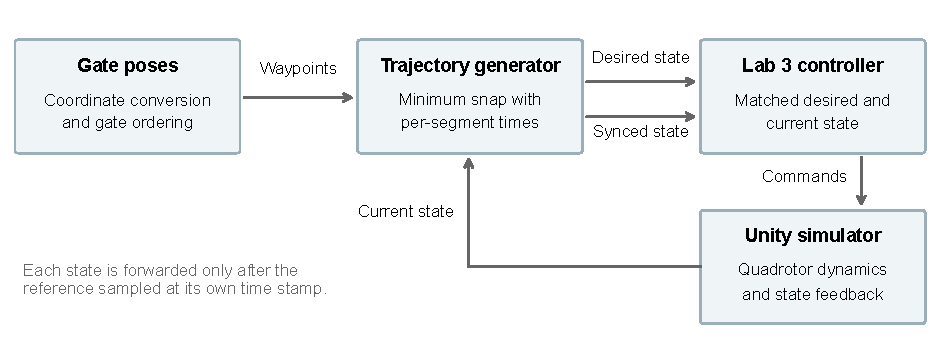
\includegraphics[width=\linewidth]{system_overview.pdf}
\caption{Implemented ROS control loop. Gate poses enter the generator on
\texttt{/desired\_traj\_vertices}. For each state received on
\texttt{/current\_state}, the generator publishes the matching
\texttt{/desired\_state} and then forwards the state on \texttt{/synced\_state},
which is the controller's state input.}
\label{fig:system}
\end{figure}

\section{Individual work}
\subsection{Deliverable 1: single-segment trajectory optimisation}
The objective is to minimise squared velocity on the normalised interval $[0,1]$:
\begin{equation}
\min_P J(P)=\int_0^1[P'(t)]^2\,dt,
\qquad P(0)=0,\quad P(1)=1.
\label{eq:single}
\end{equation}
Write $P(t)=\sum_{i=1}^N p_i t^i$. The constant coefficient is zero because
$P(0)=0$. With $\boldsymbol p=[p_1,\ldots,p_N]^T$, direct integration gives
\begin{equation}
J=\boldsymbol p^TQ\boldsymbol p,\qquad Q_{ij}=\frac{ij}{i+j-1},\qquad
A\boldsymbol p=b,\quad A=[1,\ldots,1],\quad b=1.
\label{eq:qp}
\end{equation}
$Q$ is positive definite: a nonzero coefficient vector gives a nonzero derivative
polynomial and hence a strictly positive integral of its square. Thus each feasible
equality-constrained problem has a unique minimum. A solver that defines the objective
as $\tfrac12\boldsymbol p^TH\boldsymbol p$ must use $H=2Q$.

\subsubsection{Question 1: degree one}
For $P(t)=p_1t$, the endpoint equation fixes $p_1=1$. Therefore
\begin{equation}
\boxed{P^*(t)=t,\qquad J^*=1.}
\end{equation}

\subsubsection{Question 2: degree two}
For $P(t)=p_2t^2+p_1t$, the requested matrices and objective are
\begin{equation}
Q=\begin{bmatrix}1&1\\1&4/3\end{bmatrix},\quad
A=\begin{bmatrix}1&1\end{bmatrix},\quad b=1,
\qquad J=p_1^2+2p_1p_2+\frac43p_2^2.
\end{equation}
Substituting $p_1=1-p_2$ gives $J=1+\tfrac13p_2^2$. The optimum is
$\boldsymbol p^*=(1,0)^T$, so $P^*(t)=t$ and $J^*=1$. The quadratic term
provides no cost reduction for these boundary conditions.

\subsubsection{Question 3: degree three and the Euler--Lagrange equation}
For $P(t)=p_3t^3+p_2t^2+p_1t$,
\begin{equation}
Q=\begin{bmatrix}1&1&1\\1&4/3&3/2\\1&3/2&9/5\end{bmatrix},\quad
A=\begin{bmatrix}1&1&1\end{bmatrix},\quad b=1.
\end{equation}
The Karush--Kuhn--Tucker (KKT) equations,
\begin{equation}
2Q\boldsymbol p+A^T\lambda=0,\qquad A\boldsymbol p=b,
\end{equation}
give $\boldsymbol p^*=(1,0,0)^T$ and $\lambda=-2$. Again $J^*=1$.
For the integrand $(P')^2$, the Euler--Lagrange equation is $P''=0$,
which yields the same linear trajectory. Cauchy--Schwarz also gives the global bound
\begin{equation}
J\geq\left(\int_0^1P'(t)\,dt\right)^2=[P(1)-P(0)]^2=1.
\end{equation}
Equality requires constant velocity, so increasing the degree cannot improve this result.

\subsubsection{Question 4: prescribed terminal velocity}
Adding $P'(1)=-2$ supplies a second constraint row, $[1,2,\ldots,N]$,
with $b=(1,-2)^T$. The equality-constrained minimum can be written as
\begin{equation}
\boldsymbol p^*=Q^{-1}A^T(AQ^{-1}A^T)^{-1}b.
\end{equation}

For degree two,
\begin{equation}
A=\begin{bmatrix}1&1\\1&2\end{bmatrix},\quad
b=\begin{bmatrix}1\\-2\end{bmatrix},\quad
\boldsymbol p^*=\begin{bmatrix}4\\-3\end{bmatrix}.
\end{equation}
Both coefficients are fixed by the constraints, giving
\begin{equation}
\boxed{P^*(t)=4t-3t^2,\qquad J^*=\int_0^1(4-6t)^2\,dt=4.}
\end{equation}

For degree three,
\begin{equation}
A=\begin{bmatrix}1&1&1\\1&2&3\end{bmatrix},\qquad
b=\begin{bmatrix}1\\-2\end{bmatrix}.
\end{equation}
Set $p_3=z$. The constraints give $p_1=4+z$ and $p_2=-3-2z$, so
\begin{equation}
J(z)=4+z+\frac{2}{15}z^2,\qquad J'(z)=1+\frac{4}{15}z.
\end{equation}
Its minimum occurs at $z=-15/4$, with
\begin{equation}
\boxed{P^*(t)=\frac14t+\frac92t^2-\frac{15}{4}t^3,\qquad J^*=\frac{17}{8}.}
\end{equation}
The cubic satisfies both $P(1)=1$ and $P'(1)=-2$. Its additional freedom reduces
the integrated squared velocity by $46.875\%$ relative to the quadratic. Both
trajectories overshoot the final position before returning with negative velocity
(Figure~\ref{fig:single}). These solutions minimise the cost within their specified
polynomial spaces; the linear Euler--Lagrange solution cannot satisfy the added
terminal-velocity condition.

\begin{figure}[!htbp]
\centering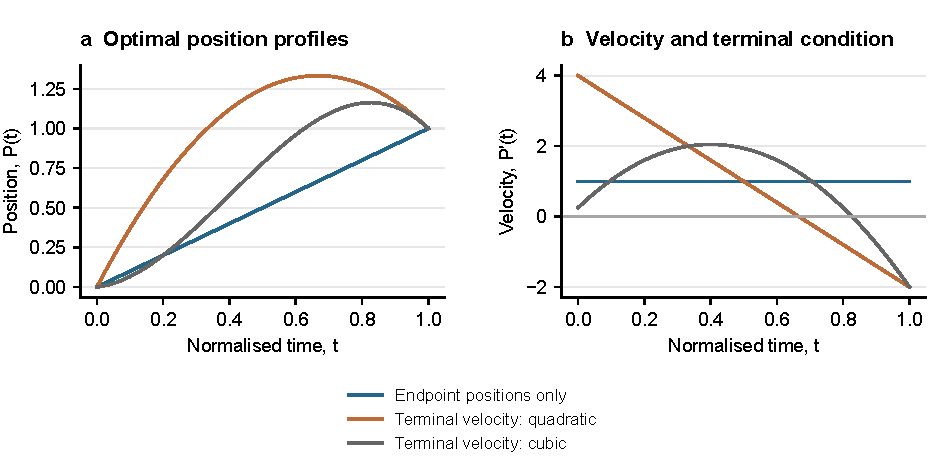
\includegraphics[width=\linewidth]{single_segment.pdf}
\caption{Exact solutions of the single-segment exercises. (a) Position profiles.
(b) Their analytic derivatives. The blue line solves the position-only problem
for degrees one, two and three. The other curves include $P'(1)=-2$; their
costs are 4 (quadratic) and $17/8$ (cubic). These are analytical curves,
not flight measurements.}
\label{fig:single}
\end{figure}

Figure~\ref{fig:objectives} shows the reduced objectives after the endpoint
equations have been eliminated. The stationary points of these one-dimensional
quadratics give the same coefficients as the matrix solution. In the terminal-velocity
problem, setting the cubic coefficient to zero recovers the degree-two solution.
\begin{figure}[!htbp]
\centering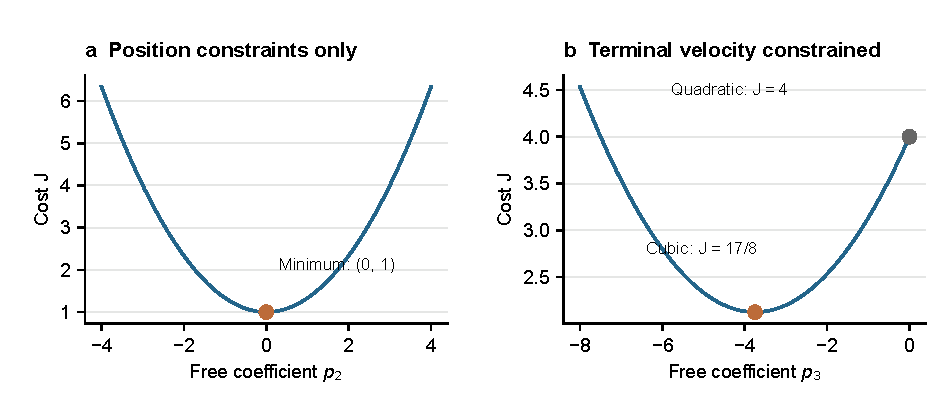
\includegraphics[width=\linewidth]{reduced_objectives.pdf}
\caption{The analytical cost landscapes. (a) For the position-only quadratic,
$J=1+p_2^2/3$ is minimised at $p_2=0$. (b) With terminal velocity $-2$,
the cubic's reduced objective is $J=4+p_3+2p_3^2/15$. Its minimum at
$p_3=-15/4$ has cost $17/8$; the point $p_3=0$ has the quadratic cost 4.}
\label{fig:objectives}
\end{figure}

\subsection{Deliverable 2: multi-segment trajectory optimisation}
All counts below refer to one scalar coordinate, prescribed waypoint positions and
fixed, strictly increasing knot times $t_0<\cdots<t_k$. Coordinates can be treated
independently when the cost is their summed squared derivative norm.

\subsubsection{Question 1: minimum snap}
For $k$ segments, the snap objective is
\begin{equation}
J=\sum_{i=1}^{k}\int_{t_{i-1}}^{t_i}[P_i^{(4)}(t)]^2\,dt.
\end{equation}
Euler--Lagrange gives $P_i^{(8)}=0$ on every open segment. Each piece therefore
has degree at most seven and eight coefficients, giving $8k$ unknowns.
Assume that position, velocity, acceleration and jerk are fixed at the overall
start and end. The conditions determining the stationary optimum are listed in
Table~\ref{tab:counts}.

\begin{table}[htbp]
\centering\small
\caption{Scalar condition count for $k$ minimum-snap segments. The free-derivative
row combines continuity constraints with natural optimality conditions.}
\label{tab:counts}
\begin{tabularx}{\linewidth}{@{}lXr@{}}
\toprule
Type & Conditions & Count\\\midrule
Waypoint & Fix both ends of each piece to the appropriate waypoint. & $2k$\\
Free derivative & Match derivatives of orders 1 to 6 across each interior knot. & $6(k-1)$\\
Fixed derivative & Specify orders 1 to 3 at the overall start and end. & $6$\\\midrule
Total & Eight conditions per polynomial piece. & $8k$\\\bottomrule
\end{tabularx}
\end{table}

There are $k+1$ physical waypoints. Each interior waypoint supplies two position
equations, one for each adjacent piece, while each overall endpoint supplies one.
For $k=3$, the counts are 6 waypoint, 12 free-derivative
and 6 fixed-derivative equations, totalling 24.

The derivative map in Figure~\ref{fig:continuity} shows where these conditions
act. Each interior position is imposed on both adjacent pieces, whereas the
free derivatives share a common value across the knot.
\begin{figure}[!htbp]
\centering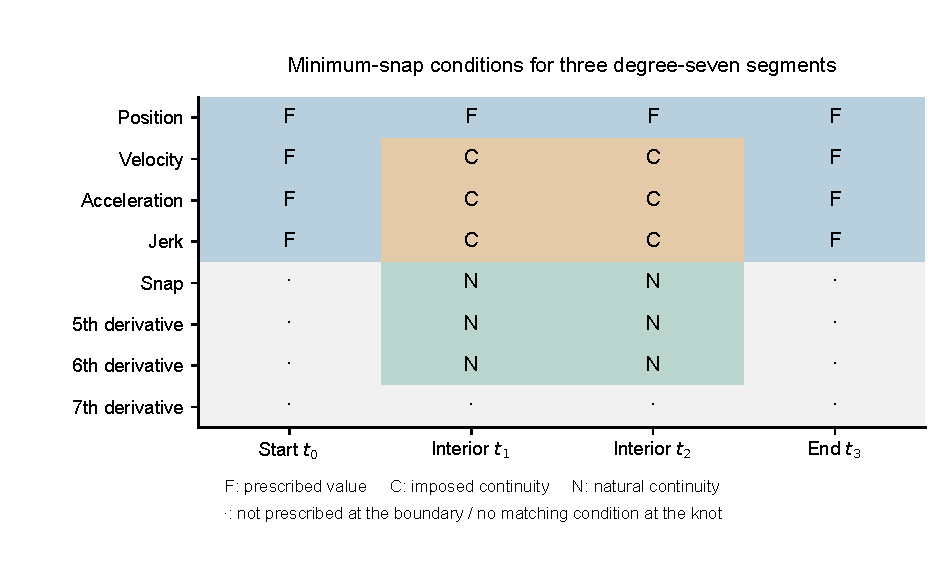
\includegraphics[width=\linewidth]{continuity_map.pdf}
\caption{Condition map for the theoretical three-segment minimum-snap problem.
F denotes a prescribed value, C an explicit continuity constraint and N a natural
continuity condition supplied by stationarity. Each interior F in the position row
represents two scalar equations. Dots identify derivative values that are not
prescribed at an endpoint, or derivatives with no knot-matching condition.}
\label{fig:continuity}
\end{figure}

Velocity, acceleration and jerk continuity define admissible trajectories. Their
common values at interior knots remain free. Minimising snap then supplies continuity
of derivatives four, five and six as natural optimality conditions. The seventh
derivative may jump because the interior positions are prescribed. Thus a QP
needs $2k+3(k-1)+6=5k+3$ explicit equality constraints; optimisation supplies the
remaining $3(k-1)$ conditions. Treating all $8k$ equations as prescribed derivative
values would remove the distinction between feasibility and optimality.

\subsubsection{Question 2: a general derivative order}
For an objective involving the squared $r$th derivative,
\begin{equation}
J=\sum_{i=1}^{k}\int_{t_{i-1}}^{t_i}[P_i^{(r)}(t)]^2\,dt,
\end{equation}
Euler--Lagrange gives $P_i^{(2r)}=0$. The degree is at most $2r-1$, with $2rk$
coefficients in total. Prescribe endpoint derivatives of orders $1,\ldots,r-1$.
The counts become
\begin{equation}
\boxed{\underbrace{2k}_{\text{waypoint}}
+\underbrace{(2r-2)(k-1)}_{\text{free derivative}}
+\underbrace{2(r-1)}_{\text{fixed derivative}}=2rk.}
\label{eq:count}
\end{equation}
The free-derivative equations match orders $1,\ldots,2r-2$ at each interior knot.
Orders $1,\ldots,r-1$ are continuity constraints; orders $r,\ldots,2r-2$ follow
from stationarity. The explicit QP has $(r+1)k+r-1$ equality constraints and
$(r-1)(k-1)$ free directions.

To obtain the natural conditions, integrate the first variation by parts $r$ times:
\begin{equation}
\frac12\delta J_i=
\left[\sum_{j=0}^{r-1}(-1)^jP_i^{(r+j)}\delta P_i^{(r-1-j)}\right]_{t_{i-1}}^{t_i}
+(-1)^r\int_{t_{i-1}}^{t_i}P_i^{(2r)}\delta P_i\,dt.
\end{equation}
At an interior waypoint, $\delta P=0$. The remaining common variations
$\delta P^{(1)},\ldots,\delta P^{(r-1)}$ are arbitrary, so their boundary terms
require continuity of orders $r,\ldots,2r-2$. The count also covers $k=1$ and
$r=1$: the corresponding interior or derivative conditions disappear.


\section{Team work}
\subsection{Deliverable 3: trajectory generation and following}
The implementation builds on the provided polynomial optimisation
library\cite{mavlib} and completes Part 0 and Parts 1.1--1.3 of the exercise.
The course contains 12 ordered gate poses. Positions convert from Unity
coordinates to the ROS world frame as
\begin{equation}
(x_R,y_R,z_R)=(x_U,z_U,y_U).
\end{equation}
For quaternion components ordered as $(x,y,z,w)$, the corresponding conversion is
$(q_{Rx},q_{Ry},q_{Rz},q_{Rw})=(-q_{Ux},-q_{Uz},-q_{Uy},q_{Uw})$.
The waypoint publisher sorts gates by their numerical index and publishes a
\texttt{PoseArray} at 5\,Hz. Figure~\ref{fig:headings} shows the converted gate
centres and their yaw directions.

\begin{figure}[!htbp]
\centering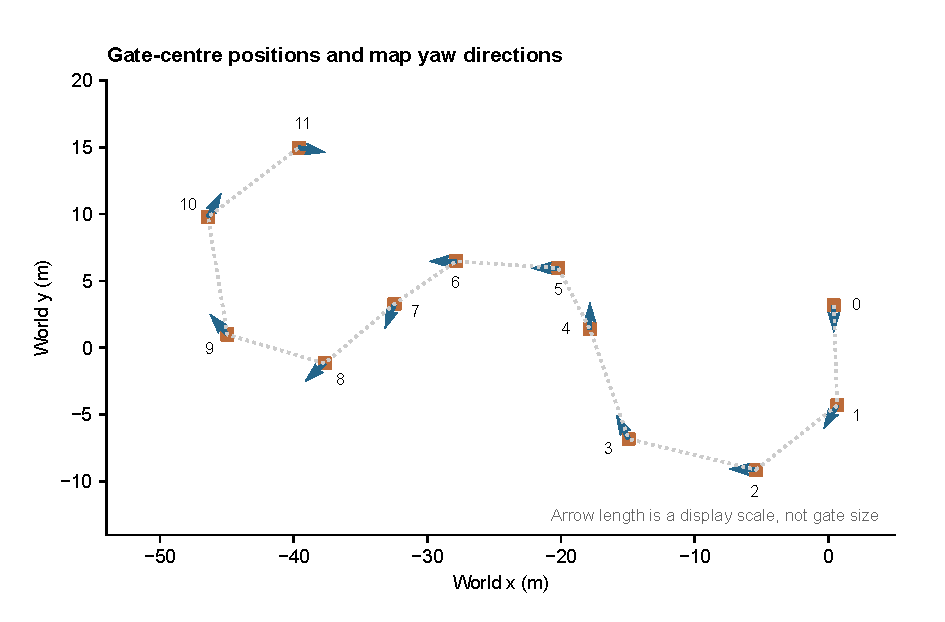
\includegraphics[width=\linewidth]{gate_headings.pdf}
\caption{Course waypoints in the ROS world frame. Squares mark the 12 gate
centres and arrows the horizontal yaw directions from the converted quaternions,
drawn at a common display length. The dotted line gives the gate order; the
optimiser chooses the smooth path between gates.}
\label{fig:headings}
\end{figure}

\subsubsection{Part 0: first-gate reference}
The simple planner takes the first gate pose, normalises its quaternion and
publishes a desired state with zero linear and angular velocity and acceleration.
A 0.01\,s timer keeps the command alive and broadcasts the desired pose in the
world frame. Empty lists and invalid first poses are rejected. In the saved hover
test the vehicle sits at $(0.423,3.165,2.374)$\,m, in front of the first gate.

\subsubsection{Part 1.1: initialise from the current state}
The follower reads position and yaw from \texttt{/current\_state} and plans only
once a valid state is available; waypoints that arrive earlier are kept until
then. The measured position becomes the first vertex, so the trajectory starts
exactly where the vehicle is. Once a trajectory exists, repeated waypoint
messages do not restart it.

\subsubsection{Part 1.2: optimise position and yaw}
The generator solves three minimum-snap problems that share one set of segment
durations: horizontal position, vertical position and yaw. Interior vertices fix
the gate position and yaw, and successive yaw angles are unwrapped with
\begin{equation}
\psi_i=\psi_{i-1}+\operatorname{atan2}
\bigl(\sin(\bar\psi_i-\psi_{i-1}),\cos(\bar\psi_i-\psi_{i-1})\bigr),
\end{equation}
where $\bar\psi_i$ is the yaw extracted from the gate quaternion. This picks the
short way round across the $\pm\pi$ boundary.

Altitude is solved on its own so that each interior gate can also fix the
vertical velocity to zero. In a joint solve the climb into one gate carries over
into the next segment; between gates 2 and 3 the joint reference rose to 4.46\,m
and struck the hall's geometry. With level gate crossings the vehicle stays between
2.0 and 3.6\,m from take-off to the finish (Figure~\ref{fig:race}c).

All three optimisers use ten coefficients per segment, so each polynomial has
degree at most nine. The library shares derivatives up to order four at interior
vertices, and \texttt{makeStartOrEnd(..., SNAP)} sets derivatives one to four to
zero at both ends. The flight trajectory therefore also fixes endpoint snap, a
slightly richer polynomial space than the degree-seven problem of Deliverable 2.

\paragraph{Per-segment time allocation.}
Segment durations decide how fast the course is flown. The library estimate
with $v_{\max}=2$\,m\,s$^{-1}$ and $a_{\max}=1$\,m\,s$^{-2}$ yields a 91.1\,s
reference. Scaling all segments uniformly until the hardest one meets its limit
is faster, but then every open straight inherits the slow timing of the tightest
turn. The generator instead treats each segment separately. For segment $i$ it
computes the stretch factor that would place that segment exactly on its
tightest limit,
\begin{equation}
s_i=\max_{t}\left\{\frac{\lVert\boldsymbol v(t)\rVert}{v_{\max}},\;
\sqrt{\frac{\lVert\boldsymbol a(t)\rVert}{a_{\max}}},\;
\sqrt{\frac{|a_z(t)|}{a_{z,\max}}}\right\},
\end{equation}
using the fact that stretching a segment by $s$ divides its velocity by $s$ and
its acceleration by $s^2$. Each iteration moves every duration toward its own
limit, $T_i\leftarrow T_i s_i^{\beta}$, re-solves the three problems, and records
the shortest allocation that satisfies all limits after a final common scaling.
Because unequal durations also reshape the path, a step is rejected and $\beta$
halved whenever a segment bends more than a 0.5\,m corridor further from its
chord than in the uniform-time solution. The separate vertical limit reflects
that a quadrotor cannot accelerate downward faster than gravity allows; without
it, a sharp climb into a level gate demanded an aggressive pitch-over at take-off.
With $v_{\max}=8$\,m\,s$^{-1}$, $a_{\max}=6$\,m\,s$^{-2}$, $a_{z,\max}=5$\,m\,s$^{-2}$,
$\beta_0=0.5$ and a 0.5\,s minimum segment time, the allocation gives an
18.91\,s reference over 95.5\,m of path.

\subsubsection{Part 1.3: publish the desired state}
The generator evaluates position, velocity, acceleration, yaw, yaw rate and yaw
acceleration at a requested time, clipped to $[0,T]$ for a trajectory of duration
$T$. The final rest pose therefore stays active after the race. Instead of using
a free-running timer, the generator samples the reference at the time stamp of
each incoming state and forwards that state on \texttt{/synced\_state} only after
publishing the matching sample. The simulation clock advances in uneven steps of
20--80\,ms, so a timer sample is typically 20--40\,ms ahead of the state the
controller pairs it with. At 8\,m\,s$^{-1}$ that offset alone is 0.16--0.32\,m of
apparent position error, which the controller would chase. Stamped sampling
removes this offset by construction. A 100\,Hz timer remains as a fallback when
states stop arriving, and the planned path is latched on \texttt{/desired\_path}
for RViz.

\subsection{Experimental configuration}
The controller gains were $k_x=14$, $k_v=6$, $k_R=12$ and
$k_\omega=2.2$, with drag compensation disabled and state and desired-state
timeouts of 1\,s. With the simulator's inertia of $J=0.1$\,kg\,m$^2$, $k_R=12$
sets an attitude bandwidth of $\sqrt{k_R/J}\approx11$\,rad\,s$^{-1}$. The build log
records seven packages built successfully, and the integration checks cover input
validation, waiting for the initial state, repeated waypoint messages, yaw
wrapping, derivative consistency and holding the final pose.

The Unity screen and RViz were recorded simultaneously at 30 frames per second,
together with a ROS bag of the run. Telemetry is sampled every 20\,ms of
simulation time; each row pairs a measured position with the
reference evaluated at the same stamp. For sample $j$ the tracking error is
\begin{equation}
e_j=\lVert\boldsymbol x_j-\boldsymbol x_{d,j}\rVert_2,\qquad
e_{\mathrm{RMS}}=\sqrt{\frac{1}{|\mathcal A|}\sum_{j\in\mathcal A}e_j^2},
\end{equation}
where the active set $\mathcal A$ holds the samples taken before the
reference reaches its end. The remaining samples cover 10.8\,s of the final
hold. For gate $i$ with centre $\boldsymbol g_i$, the gate-centre distance is
$d_i=\min_j\lVert\boldsymbol x_j-\boldsymbol g_i\rVert_2$, taken at time
$t_i=t_{\arg\min_j\lVert\boldsymbol x_j-\boldsymbol g_i\rVert_2}$.

\subsection{An 18.9-second race through all 12 gates}
Figure~\ref{fig:race} summarises the race. The vehicle leaves the floor, passes
the gates in order at 1.2--2.5\,s intervals and stops at the last gate 18.91\,s
after the start, an average speed of 5.1\,m\,s$^{-1}$. The speed trace shows the
effect of per-segment allocation: on the long sweep from gate 2 to gate 4 and
again from gate 10 to the finish the reference runs at 7.0--7.2\,m\,s$^{-1}$,
close to the 8\,m\,s$^{-1}$ limit, and it slows to 3.3\,m\,s$^{-1}$ only in the
two tightest turns, between gates 4 and 5 and between gates 9 and 10. Recorded speed follows the reference so closely that
the two curves overlap, and altitude stays level through each gate. The
simulator logged no collision after take-off.

\begin{figure}[!htbp]
\centering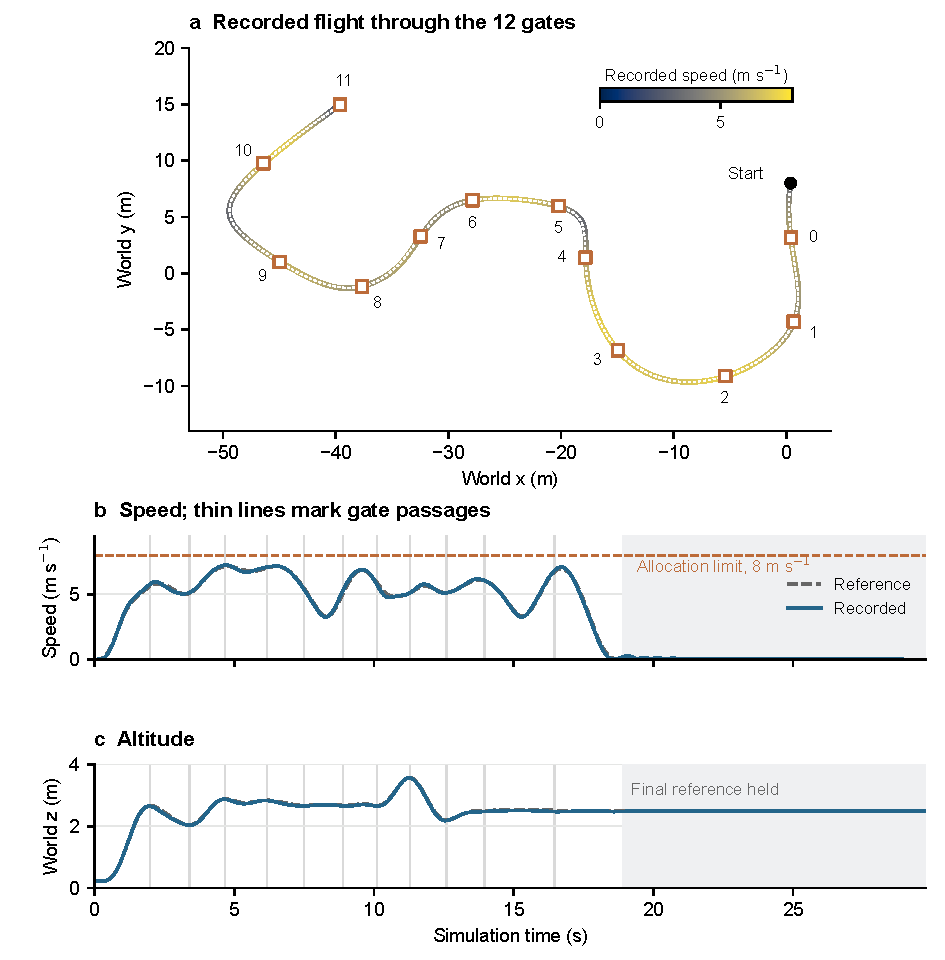
\includegraphics[width=\linewidth]{race_overview.pdf}
\caption{The recorded Unity race. (a) Horizontal path coloured by measured
speed, with the reference dashed in white and gate centres as squares; axes use
equal scale. (b) Reference and measured speed; thin vertical lines mark the
closest approach to gates 0--10 and the dashed line is the allocation limit.
(c) Reference and measured altitude. Shading marks the final hold. All
telemetry samples are shown.}
\label{fig:race}
\end{figure}

\begin{figure}[!htbp]
\centering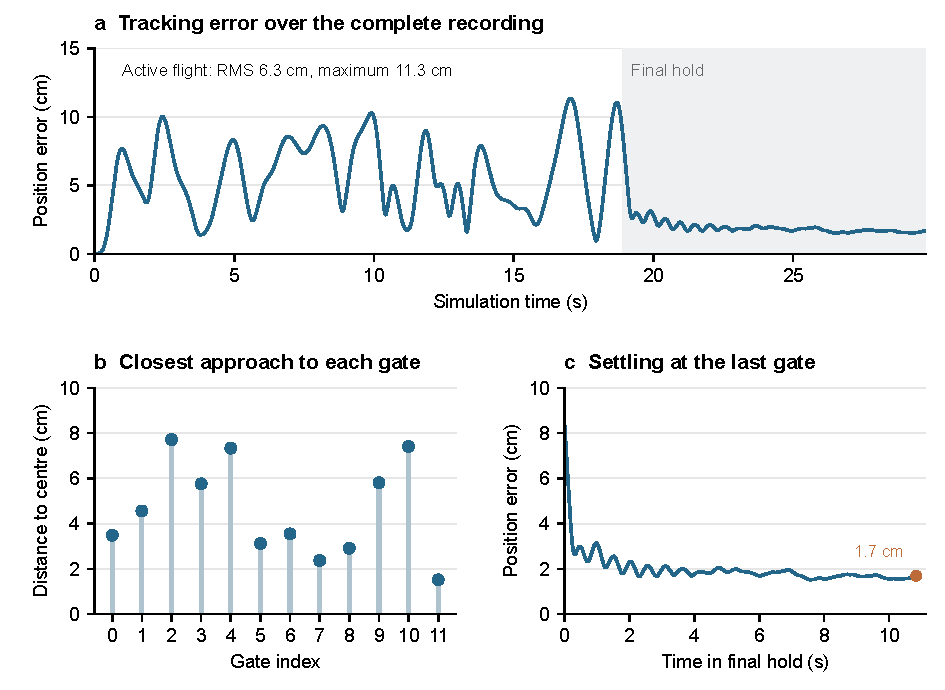
\includegraphics[width=\linewidth]{tracking_accuracy.pdf}
\caption{Tracking accuracy. (a) Euclidean position error for every sample; the
shaded interval is the final hold. (b) Minimum distance from the measured
position to each gate centre. (c) Error during the final hold, with the last
sample marked.}
\label{fig:accuracy}
\end{figure}

\subsection{Centimetre-level tracking}
Over the active race the RMS tracking error is 6.3\,cm, the median 5.4\,cm and
the maximum 11.3\,cm (Figure~\ref{fig:accuracy}a), at speeds above 7\,m\,s$^{-1}$
and tilt angles up to 35$^\circ$. Per axis, the RMS residuals are 4.6\,cm in $x$,
3.6\,cm in $y$ and 2.2\,cm in $z$; the vertical axis is the most accurate, which
reflects the level gate crossings.

Every gate is passed close to its centre (Figure~\ref{fig:accuracy}b and
Table~\ref{tab:gates}). The largest gate-centre distance is 7.7\,cm at gate 2,
and seven of the twelve gates are passed within 5\,cm. The local views in
Appendix~\ref{sec:gateatlas} show that the measured path and the reference cross
each gate together and level.

When the reference stops, the error falls from 8.5\,cm to about 3\,cm within
half a second and settles at 1.5--2.5\,cm (Figure~\ref{fig:accuracy}c). The last sample is
1.7\,cm from the final gate centre, 10.8\,s into the hold.

\begin{table}[htbp]
\centering\small
\caption{Measured performance of the recorded race.}
\label{tab:metrics}
\begin{tabular}{@{}lr@{}}
\toprule
Quantity & Value\\\midrule
Reference duration / path length & 18.91\,s / 95.5\,m\\
Mean / peak measured speed & 5.1 / 7.3\,m\,s$^{-1}$\\
Peak tilt & 34.8$^\circ$\\
RMS / median / maximum tracking error & 6.3 / 5.4 / 11.3\,cm\\
Largest gate-centre distance & 7.7\,cm\\
Final position error after 10.8\,s hold & 1.7\,cm\\
High-frequency tilt (RMS) & 0.10$^\circ$\\
\bottomrule
\end{tabular}
\end{table}

\begin{table}[htbp]
\centering\small
\caption{Closest approach to each gate centre. Gate 11 is the finish; its closest
approach falls in the final hold, where the vehicle settles onto it.}
\label{tab:gates}
\begin{tabular}{@{}rrr@{\hspace{10mm}}rrr@{}}
\toprule
Gate & Time (s) & Distance (cm) & Gate & Time (s) & Distance (cm)\\\midrule
0 & 2.00 & 3.5 & 6 & 10.10 & 3.5\\
1 & 3.40 & 4.6 & 7 & 11.28 & 2.4\\
2 & 4.68 & 7.7 & 8 & 12.60 & 2.9\\
3 & 6.18 & 5.8 & 9 & 13.96 & 5.8\\
4 & 7.50 & 7.3 & 10 & 16.46 & 7.4\\
5 & 8.90 & 3.1 & 11 & 26.50 & 1.5\\\bottomrule
\end{tabular}
\end{table}

\subsection{Smooth attitude at racing speed}
The race asks for large, fast attitude changes: roll swings between $-31^\circ$
and $+35^\circ$ within a few seconds (Figure~\ref{fig:attitude}a). The relevant
quality measure is therefore not the size of the tilt but whether it is clean.
To isolate jitter, roll and pitch are each fitted with a local quadratic over a
0.5\,s window and the residual is combined into a tilt jitter,
$\sqrt{\delta\phi^2+\delta\theta^2}$. In this race the jitter has an RMS of
0.10$^\circ$ and never exceeds 0.8$^\circ$.

Figure~\ref{fig:attitude}b compares this with an earlier flight that used a
timer-sampled reference. There, jitter reaches 2.8$^\circ$ and averages
0.49$^\circ$, five times more. That earlier flight also used uniform time scaling and softer gains. The
tuning runs in Table~\ref{tab:design} isolate the timing change: with every
other setting fixed, stamped sampling alone reduced jitter from 0.45$^\circ$ to
0.04$^\circ$ RMS and tracking error from 7.4 to 5.1\,cm.

\begin{figure}[!htbp]
\centering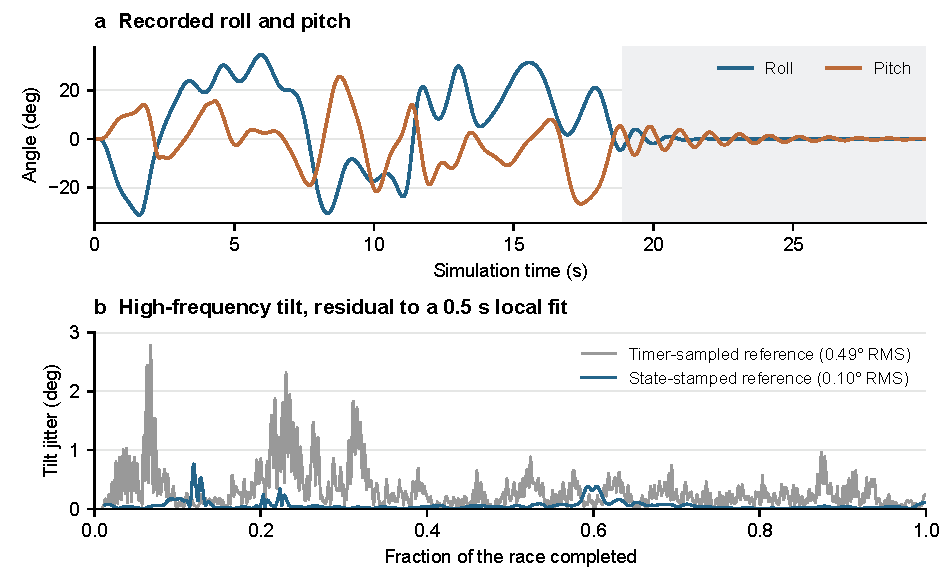
\includegraphics[width=\linewidth]{attitude_smoothness.pdf}
\caption{Attitude during the race. (a) Measured roll and pitch from the recorded
quaternions (ZYX convention); shading marks the final hold. (b) Tilt jitter,
the residual of roll and pitch after a local quadratic fit over 0.5\,s, for this
race and for an earlier 25.5\,s flight with a timer-sampled reference. Time is
normalised by each reference duration; the legend gives the active-flight RMS.}
\label{fig:attitude}
\end{figure}

\begin{table}[htbp]
\centering\small
\caption{Tuning runs on the same course and simulator that led to the final
configuration. Jitter is the RMS tilt jitter defined above; error is the RMS
tracking error.}
\label{tab:design}
\begin{tabularx}{\linewidth}{@{}Xrrr@{}}
\toprule
Configuration & Duration & Jitter & Error\\\midrule
Uniform scaling ($v_{\max}=10$, $a_{\max}=8$), timer-sampled reference & 25.5\,s & 0.45$^\circ$ & 7.4\,cm\\
Same, with stamped sampling & 25.5\,s & 0.04$^\circ$ & 5.1\,cm\\
Uniform scaling pushed to $v_{\max}=14$, $a_{\max}=12$ & 20.2\,s & 0.76$^\circ$ & 9.8\,cm\\
Per-segment allocation ($v_{\max}=8$, $a_{\max}=6$), $k_R=12$ & 18.9\,s & 0.09$^\circ$ & 6.0\,cm\\
\bottomrule
\end{tabularx}
\end{table}

Table~\ref{tab:design} also shows where the speed comes from. Pushing uniform
scaling to much higher limits shortens the race only to 20.2\,s, and it does so by
making the first climb so steep that the vehicle pitched to 84$^\circ$ at
take-off. Per-segment allocation reaches 18.9\,s with lower limits and with
jitter at the level of the synchronised baseline. The gain $k_R=12$ was chosen
over a stiffer $k_R=22$: the stiffer setting tracked marginally better on a good
run, but in repeated runs it occasionally broke into attitude
oscillations of up to 15$^\circ$ in hard turns, which never happened with $k_R=12$.

\subsection{Simulator and RViz views}
Figure~\ref{fig:video} places the telemetry in the rendered scene. The onboard
camera shows the vehicle banking through the course, each gate turning from red
to green as it is passed, and the vehicle holding at the finish. The RViz view,
recorded at the same time, overlays the planned path and the measured path; at
this scale they are indistinguishable.

\begin{figure}[!htbp]
\centering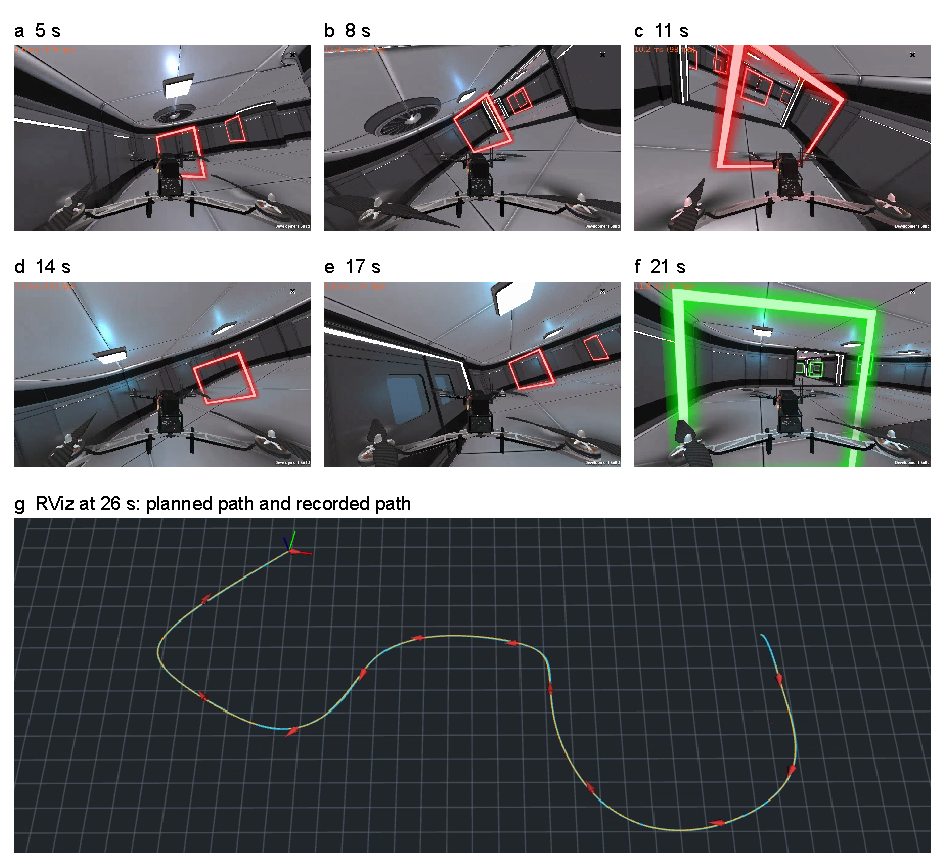
\includegraphics[width=\linewidth]{race_video.pdf}
\caption{Frames from the simultaneous screen recordings. (a--f) Unity view at
5, 8, 11, 14, 17 and 21\,s of video playback, full frames without colour
adjustment. (g) RViz at 26\,s, cropped to the 3D view: planned trajectory,
measured path, gate poses as red arrows and the desired frame at the finish.
Playback time includes the take-off preparation and is not aligned with the
telemetry clock.}
\label{fig:video}
\end{figure}

\section{Discussion}
\subsection{Polynomial freedom and boundary conditions}
The single-segment solutions show when a higher polynomial degree pays off.
With position constraints alone, constant velocity already reaches the global
lower bound. A terminal-velocity condition changes the feasible set: a cubic can
redistribute velocity over the interval and lowers the cost from 4 to $17/8$.
The overshoot in Figure~\ref{fig:single} is the price of arriving at the final
point with negative velocity. Boundary conditions, more than polynomial degree,
determine what extra coefficients are worth.

For multiple segments, the split between explicit constraints and natural
conditions explains how the optimiser sets the free derivatives at each
waypoint. The flight implementation uses the same idea deliberately: it adds one
explicit constraint, zero vertical velocity at each gate, exactly where the
natural solution produced an unwanted climb, and leaves the remaining
derivatives to the optimiser.

\subsection{What makes the race fast and clean}
Two choices outside the polynomial optimisation carry most of the result. Time
allocation is the speed lever: per-segment durations let the reference run near
its limits on open sections and slow down only where the geometry demands it,
which gives a shorter race than uniform scaling at much higher limits. Timing is
the smoothness lever: at racing speed a few tens of milliseconds between a state
and its reference look like decimetres of error to the controller, and sampling
the reference at the state's own stamp removes that error source entirely. With
both in place, a controller tuned for moderate bandwidth tracks a
7\,m\,s$^{-1}$ reference to within a few centimetres.

\section{Conclusions}
The analytical exercises connect polynomial coefficients to boundary conditions
and separate the constraints a minimum-snap solver must impose from those that
optimality provides. The ROS follower carries this formulation to spatial
waypoints and unwrapped yaw, allocates segment time against speed and
acceleration limits, and delivers each reference sample at the time of the state
it is paired with. In Unity, the Lab 3 controller flies the 12-gate course in
18.91\,s, passes every gate within 7.7\,cm of its centre, tracks the reference
with 6.3\,cm RMS error and smooth attitude, and settles 1.7\,cm from the finish.

\begingroup\small\setlength{\bibsep}{2pt}\begin{thebibliography}{9}
\bibitem{lab4} MIT Visual Navigation for Autonomous Vehicles.
\emph{Lab 4: Exercises}, 2023 course materials.
\url{https://vnav.mit.edu/labs_2023/lab4/exercises.html}.
Accessed 10 October 2026.
\bibitem{mavlib} ETH Zurich Autonomous Systems Lab.
\emph{mav\_trajectory\_generation: Polynomial trajectory generation and optimisation}.
\url{https://github.com/ethz-asl/mav_trajectory_generation}.
Library documentation and the implementation distributed with the laboratory.
Accessed 10 October 2026.
\end{thebibliography}\endgroup

\appendix
\section{Gate-by-gate views}
\label{sec:gateatlas}
Figures~\ref{fig:glocalfirst} and~\ref{fig:glocallast} show the reference and
measured path around each gate. The horizontal coordinate
$s=\cos\psi_i(x-x_i)+\sin\psi_i(y-y_i)$ is the offset along the map yaw of gate
$i$, and the vertical coordinate is $z-z_i$. Each panel covers 1\,s on either side
of the closest approach (for the finish gate, of the moment the reference ends),
and its title gives the full 3D gate-centre distance.

\begin{figure}[!htbp]
\centering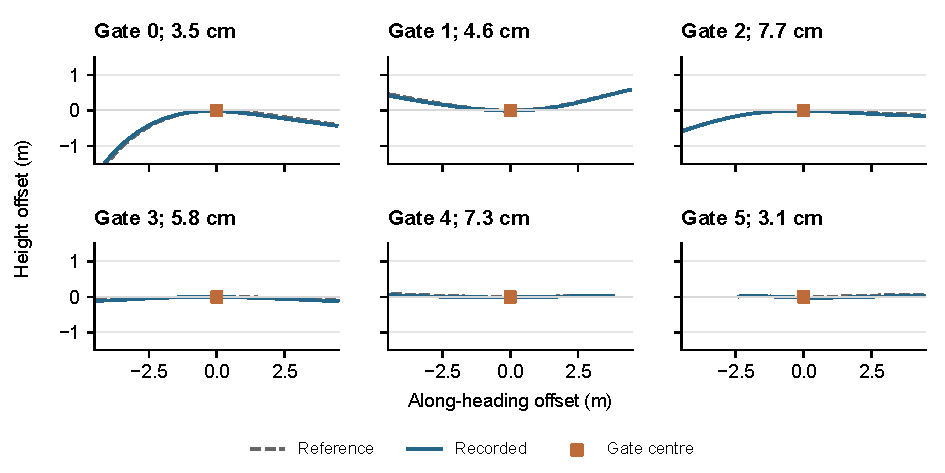
\includegraphics[width=\linewidth]{gate_local_00_05.pdf}
\caption{Reference and measured path around gates 0--5, projected onto the gate
heading and height. The square marks the gate centre; samples within $\pm1$\,s of
the closest approach and within $\pm4.5$\,m along the heading are shown.}
\label{fig:glocalfirst}
\end{figure}
\begin{figure}[!htbp]
\centering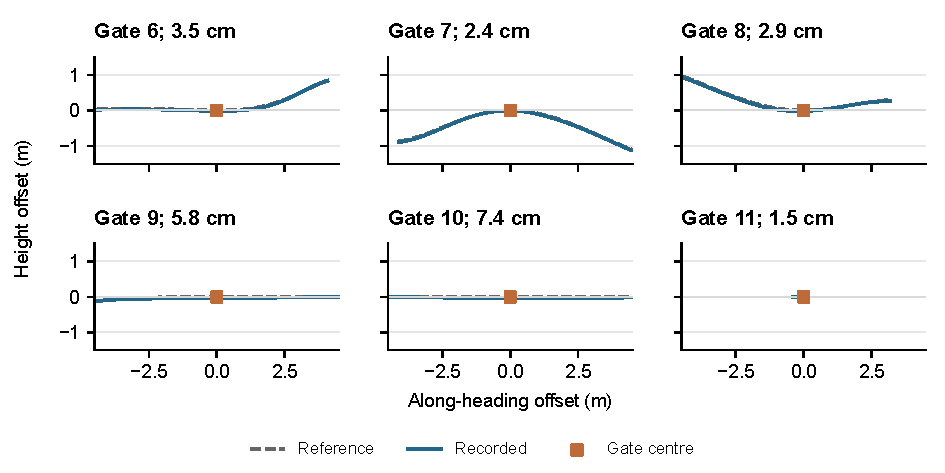
\includegraphics[width=\linewidth]{gate_local_06_11.pdf}
\caption{The same views for gates 6--11. Gate 11 is the finish, where the vehicle
decelerates to rest on the gate centre.}
\label{fig:glocallast}
\end{figure}
\end{document}
